\chapter{Search Problems \& Uninformed Search}

\section{Search Problems}

\subsection{Review}

In order to formalize a problem as a search problem, we need to define the following:

\begin{listo}
    \item \term{eState Space}: A state is a representation of a configuration of the problem domain. The state space is the set of all states included in our model of the problem.
    \item \term{Initial State}: The starting configuration.
    \item \term{Goal State}: The configuration one wants to achieve. 
    \item \term{Actions} (or \term{State Space Transitions}): Allowed changes to move from one state to another.
\end{listo}

Optionally, we may use the following:
\begin{listo}
    \item \term{Costs}: Representing the cost of moving from state to state.
    \item \term{Heuristics}: Help guide the heuristic process
\end{listo}

\begin{example}[Make Change]
    We start with $0$ cents and we want to reach some number of cents between $[0, 5, 10, 15, ..., 500]$ using the least number of coins. We can add $5, 100, 25, 100$, or $200$ cents.

    Search problem formulation with the goal of $X$ cents:
    \begin{listu}
        \item States: Integers between 0 and 500 that are divisible by 5.
        \item Initial State: 0
        \item Goal State: $X$
        \item Actions: Add 5, 10, 25, 100, or 200
    \end{listu}
\end{example}

\subsection{Questions}

\begin{listo}
    \item Sudoku is a popular number puzzle that works as follows: we are given a $9 \times 9$ square grid; some squares have numbers, while some are blank. Our objective is to fill in the blanks with numbers from $1 - 9$ such that each row, column, and the highlighted $3 \times 3$ squares contain no duplicate entries (see Figure 1).
    
    % TODO: Insert Figure 1 and Figure 2

    Sudoku puzzles can be solved easily after being modelled as a CSP (which will be covered later in the course). We will consider the problem of generating Sudoku puzzles. In particular, consider the following procedure: start with a completely full number grid (see Figure 2), and iteratively make some squares blank. We continue blanking out squares as long as the resulting puzzle can be completed in at least one way.

    Complete the following:
    
    \begin{listu}
        \item Give the representation of a state in this problem.

        \begin{solution}
            A partial valis solution matrik $M \in \{ 0, \dots, 9 \}$. 
        \end{solution}

        \item Using the state representation defined above, specify the initial state and goal state(s).

        \begin{solution}
            \null

            \textbf{Initial State:} A complete filled grip. All rows, columns, and $3 \times 3$ squares contain $\{ 1, 2, \dots, 9 \}$. 

            \textbf{Goal State:} Any state that can be completed in at least one way.
        \end{solution}

        \item Define its actions.

        \begin{solution}
            \[
                M - E_{ij}(a)
            \] where $E_{ij}(a)$ is a matrix of all zero except for the $i$th row and $j$th column, which is $a = M[i, j] \neq 0$.
        \end{solution}

        \item Using the state representation and actions defined above, specify the transition function $T$. (In other words, when each of the actions defined above is applied to a current state, what is the resulting state?)
        
        \begin{solution}
                $T(M - E_{ij}(a)) = M - E_{ij}(a)$
        \end{solution}
    \end{listu}

    \item Assuming that ties (when pushing to the frontier) are broken based on alphabetical order, specify the order of the nodes that would be explored by the following algorithms. Assume that $S$ is the initial node, while $G$ is the goal node. You should express your answer in the form $S - B - A - F - G$ (i.e. no spaces, all uppercase letters, delimited by the dash ($-$) character), which, for example, corresponds to the exploration order of $S, B, A, F$, then $G$.

    \begin{figure}[ht!]
        \centering

        \tikzexternalenable
        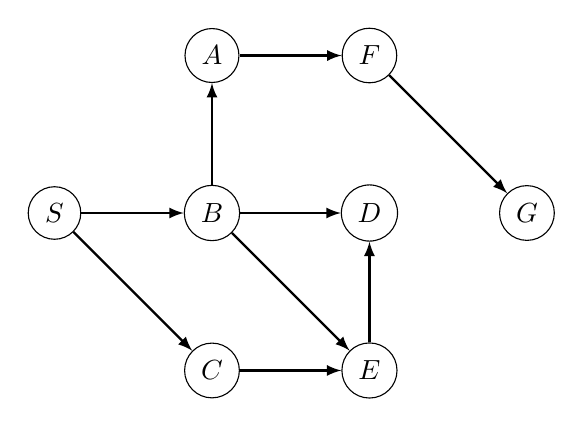
\begin{tikzpicture} [
            every node/.style = {draw=black, circle},
        ]

            \node (S) at (0,  0) {$S$};
            \node (A) at (2,  2) {$A$};
            \node (B) at (2,  0) {$B$};
            \node (C) at (2, -2) {$C$};
            \node (D) at (4,  0) {$D$};
            \node (E) at (4, -2) {$E$};
            \node (F) at (4,  2) {$F$};
            \node (G) at (6,  0) {$G$};

            \draw[thick,-latex] (S) -- (B);
            \draw[thick,-latex] (S) -- (C);
            \draw[thick,-latex] (A) -- (F);
            \draw[thick,-latex] (B) -- (A);
            \draw[thick,-latex] (B) -- (D);
            \draw[thick,-latex] (B) -- (E);
            \draw[thick,-latex] (C) -- (E);
            \draw[thick,-latex] (E) -- (D);
            \draw[thick,-latex] (F) -- (G);
        \end{tikzpicture}
        \tikzexternaldisable
        
        \caption{Graph for question 2(b).}
    \end{figure}

    \begin{listo}
        \item Depth-First Search with no cycle-checking (aka tree-based) implementation.

        \begin{solution}
            $S - C - E - D - B - E - D - A - F - G$
        \end{solution}

        \item Breadth-First Search with no cycle-checking (aka tree-based) implementation.

        \begin{solution}
            $S - B - C - A - D - E - F - G$
        \end{solution}

        \item Breadth-First Search with cycle-checking (aka graph-based) implementation.

        \begin{solution}
            $S - B - C - A - D - E - F - G$
        \end{solution}
    \end{listo}

    \item \begin{listo}
        \item The \textbf{Breadth-First Search} algorithm is complete if the state space has infinite depth but finite branching factor.
        
        Determine if the statement above is True or False, and provide a rationale.

        \begin{solution}
            True. 

            Completenes of BFS means whenever there is a path from the initial path to the goal, BFS will find it. 

            Exisance of a path means goal exist in a finite depth, hence BFS will reach it given a finite branching factor.
        \end{solution}

        \item The \textbf{Breadth-First Search} algorithm can be complete even if zero step costs are allowed.

        Determine if the statement above is True or False, and provide a rationale

        \begin{solution}
            True. 

            BFS is complete as long as state space has finite branching factor. 
        \end{solution}

        \item Given that a goal exists within a finite search space, the \textbf{Breadth-First Search} algorithm is cost-optimal if all step costs from the initial state are non-decreasing in the depth of the search tree. That is, for any given level of the search tree, all step costs are greater than the step costs in the previous level.

        Determine if the statement above is True or False, and provide a rationale

        \begin{solution}
            False. 
            
            Consider the following counter example, arbitrary alphabetic order results in $A$ reached before $B$. 

            \begin{figure}[ht!]
                \centering

                \tikzexternalenable
                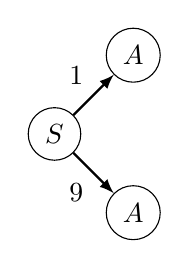
\begin{tikzpicture}
                    \node[draw, circle] (S) at (0,  0) {$S$};
                    \node[draw, circle] (A) at (1, -1) {$A$};
                    \node[draw, circle] (B) at (1,  1) {$A$};

                    \draw[thick,-latex] (S) -- (A) node[midway, below left] {$9$};
                    \draw[thick,-latex] (S) -- (B) node[midway, above left] {$1$};
                \end{tikzpicture}
                \tikzexternaldisable
            \end{figure}
        \end{solution}
    \end{listo}

    \item Prove that the \textbf{Uniform Cost Search} algorithm is cost-optimal as long as each step cost exceeds some small positive constant $\epsilon$.

    \begin{solution}
        \begin{proof}
            WTS UCS is optimal as long as each step cost exceeds positive value $\epsilon$. 

            Given that each stap cost exceeds $\epsilon$, completenemss can be assumed 

            \begin{listu}
                \item when UCS expands a node $n$, the optimal path to that node has been found. If not, there would be another node $n'$ on the optimal path from the start node to $n$ ($n'$). Bt definition it will have a lower cost than $n$.
                
                Contradition because it was not selected. 

                \item If step costs are non-negative, path never get shorter as nodes are added. Thus, UCS expands nodes in the order of the optimnal path cost. 
            \end{listu}
        \end{proof}
    \end{solution}
\end{listo}